\documentclass[12pt, letterpaper]{article}
\usepackage{graphicx}
\usepackage{caption}
\usepackage[hidelinks]{hyperref}
\usepackage{color}
\usepackage{listings}
\usepackage{array}
\usepackage{hhline}
\usepackage{multirow}
\graphicspath{{images/}}
\newcounter{nalg}[section] % defines algorithm counter for chapter-level
\renewcommand{\thenalg}{\thesection .\arabic{nalg}} %defines appearance of the algorithm counter
\DeclareCaptionLabelFormat{algocaption}{Algorithm \thenalg} % defines a new caption label as Algorithm x.y

\lstnewenvironment{algorithm}[1][] %defines the algorithm listing environment
{   
    \refstepcounter{nalg} %increments algorithm number
    \lstset{ %this is the stype
        mathescape=true,
        frame=tB,
        numbers=left, 
        numberstyle=\tiny,
        basicstyle=\scriptsize, 
        keywordstyle=\color{black}\bfseries\em,
        keywords={,input, output, return, datatype, function, in, if, else, foreach, while, begin, end, } %add the keywords you want, or load a language as Rubens explains in his comment above.
        numbers=left,
        xleftmargin=.04\textwidth,
        #1 % this is to add specific settings to an usage of this environment (for instnce, the caption and referable label)
    }
    \captionsetup{labelformat=algocaption,labelsep=colon} %defines the caption setup for: it ises label format as the declared caption label above and makes label and caption text to be separated by a ':'
}
{}
\begin{document}
    \begin{titlepage}
    \begin{center}
        \vspace*{1cm}
            
        \Huge
        \textbf{Final Report}
            
        \vspace{0.5cm}
        \LARGE
        Thermal Scanning App
            
        \vspace{1.5cm}
            
        \textbf{Colter Roche, Jose Bastardo}
            
        \vfill
          
        \Large
        Senior Design 1\\
        COP4934C.01\\
        \today
            
    \end{center}
\end{titlepage}
    \newpage
    \tableofcontents
    \newpage
    \listoftables
    \listoffigures
    \newpage
    \section{Introduction}
    \paragraph{}
    Corserva is a managed IT service provider that develops and sells custom software and 
    hardware solutions. Corserva's customers include hospitality and other in-person focused 
    related businesses. Official CDC guidelines to businesses encourage taking steps to prevent 
    the spread of Covid-19 among employees and customers, including temperature checks. Corserva 
    has sponsored this project to produce a thermal screening solution capable of processing 
    people quickly and without requiring user interaction to minimize additional contact.
    \paragraph{}
    The scope of this project is to produce an application and companion mobile application to 
    measure and report high temperatures of people passing through the system. The thermal 
    camera will use an auto calibration system to increase accuracy of readings. Mobile 
    application to smooth the onboarding process and provide reports to users.
    \paragraph{}
    The business scope is to provide business with a kiosk and mobile app
    system that will make it easier for them to maintain safety precautions during
    the current Covid 19 pandemic while also increasing the speed in which staff and customers 
    can enter their place of business.
    \section{Functional Decomposition}
    \begin{figure}[h!]
        \centering
        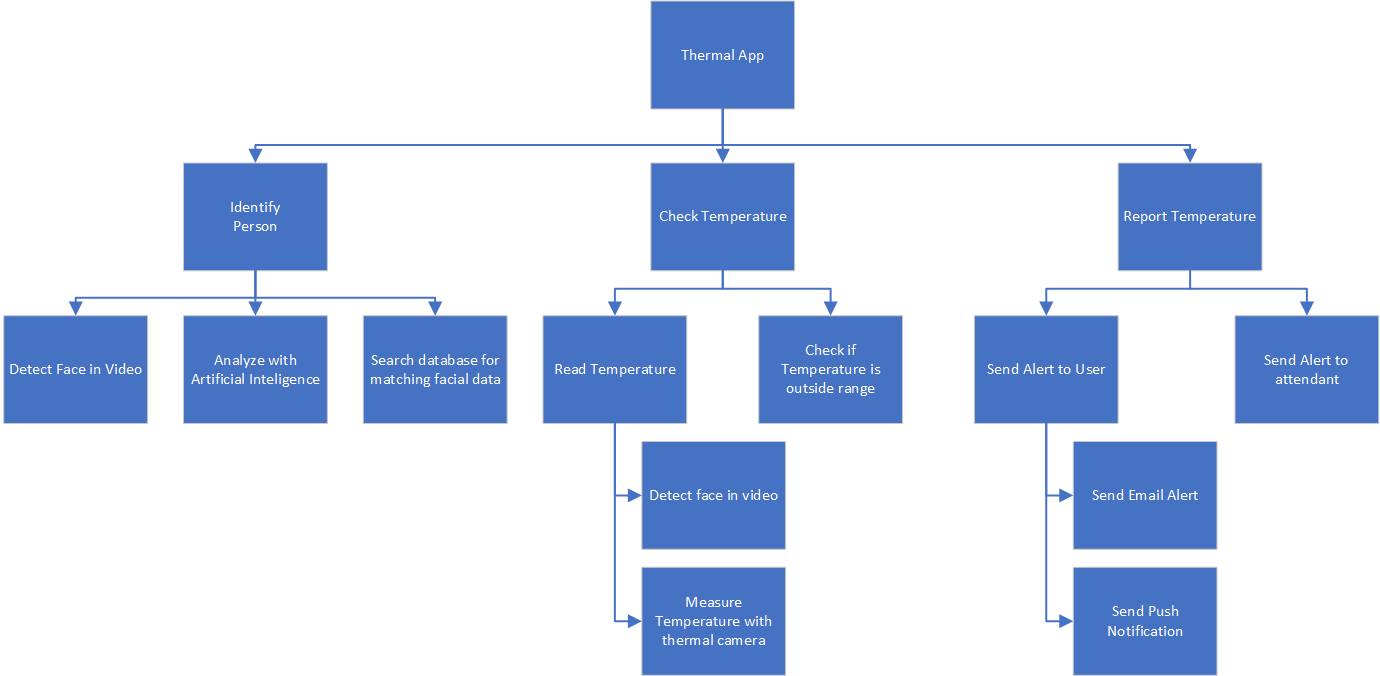
\includegraphics[width=0.8\textwidth]{Function diagram-Thermal App.png}
        \caption{Functional Decomposition Diagram - Thermal scanner}
    \end{figure}
    \begin{figure}[h!]
        \centering
        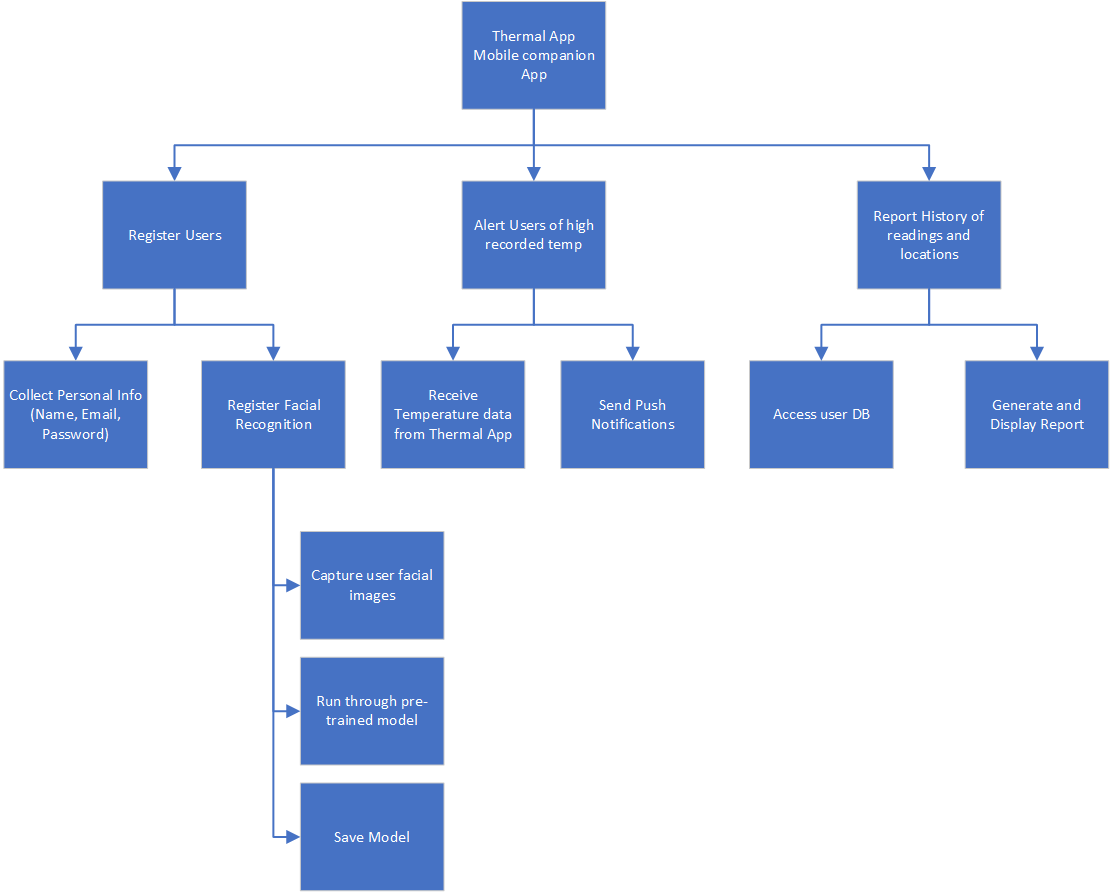
\includegraphics[width=0.8\textwidth]{Function diagram-Mobile Comapanion App.png}
        \caption{Functional Decomposition Diagram - Comapanion App}
    \end{figure}
    \newpage
    \section{Data Flow and Application Structure}
    \begin{figure}[h!]
        \centering
        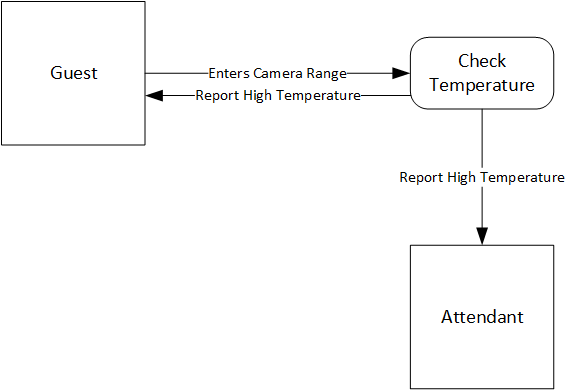
\includegraphics[width=0.8\textwidth]{DFD Top Level.png}
        \caption{Top Level Data Flow Diagram}
    \end{figure}
    \begin{figure}[h!]
        \centering
        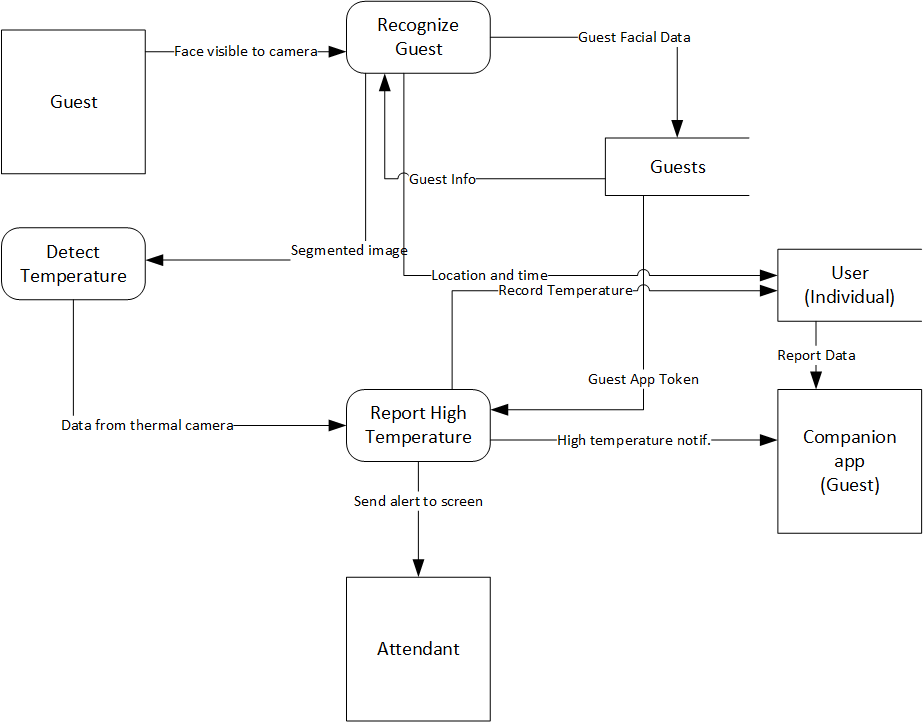
\includegraphics[width=0.8\textwidth]{DFD Level 1.png}
        \caption{Level 1 Data Flow Diagram}
    \end{figure}
    \begin{figure}[h!]
        \centering
        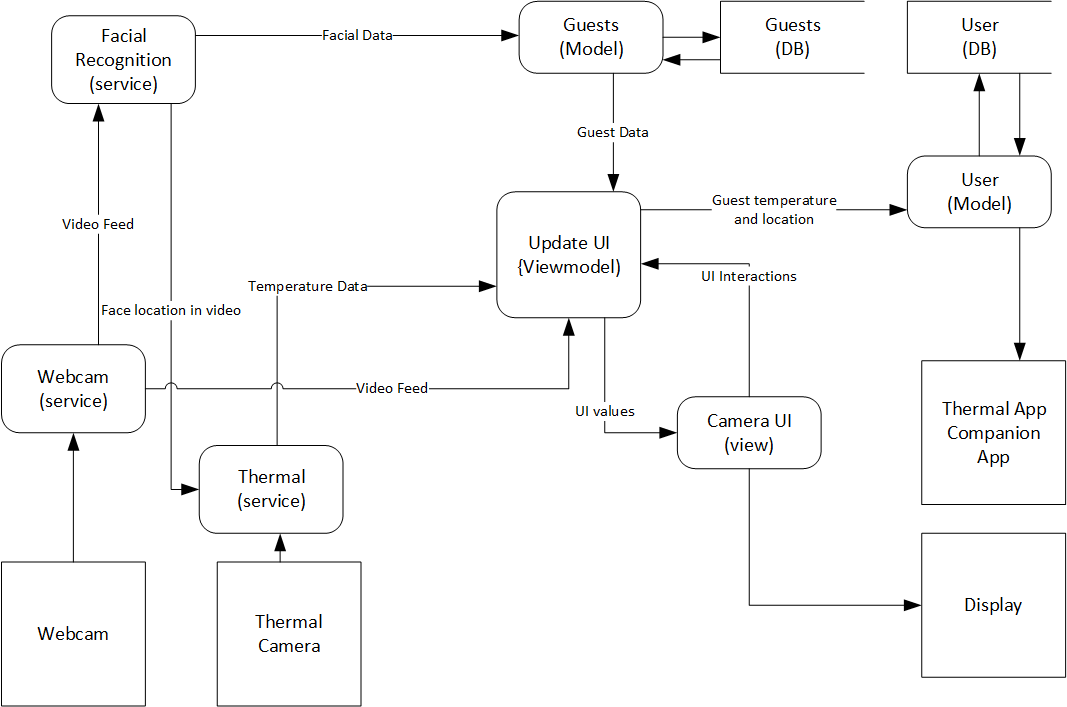
\includegraphics[width=0.8\textwidth]{DFD Level 2.png}
        \caption{Level 2 Data Flow Diagram}
    \end{figure}    
    \section{User Stories and Tasks}
    \begin{table}[ht!]
        \begin{center}
        \begin{tabular}{|>{\centering \arraybackslash}m{3.7cm}|>{\centering \arraybackslash}m{8.5cm}|}
            \hline
            Epic & User Story\\
            \hline
            \multirow{4}{3cm}{Provide facial recognition for user identification and measure user temperature}
                &As a user, I want the system to recognize me in under 2 seconds so I can save time\\\hhline{~-} 
                &As a kiosk attendant, I want to see a confirmation that the user is recognized, for security purposes\\\hhline{~-} 
                &As a kiosk attendant, I want temp measurements to be accurate withing a degree, so I do not have to check extra people/miss people\\\hhline{~-} 
                &As a kiosk attendant, I want the thermal camera to self-calibrate, to avoid the need for time consuming troubleshooting\\
            \hline
            \multirow{3}{3cm}{Provide notifications and reports to users and attendants}
                &As a kiosk attendant, I should be alerted if a registered user is detected with a high temperature to perform a manual temperature check\\\hhline{~-} 
                &As a kiosk attendant, I should be alerted if a person is not recognized as a registered user\\\hhline{~-} 
                &As a user, I should be alerted if my temperature is too high\\\hhline{~-}
            \hline
            \multirow{3}{3cm}{Provide a user onboarding system}
                &As a user, I want to register through a mobile app, for easier remote registration\\\hhline{~-} 
                &As a user, I want to register facial data through the app, so I can skip in person registration\\\hhline{~-} 
                &As a system admin, I want to have control over what information is collected from users and how long the data is stored, to increase security\\\hhline{~-} 
            \hline
        \end{tabular}
        \end{center}
        \caption{Epics and User Stories}
        \label{tab:multicol}
    \end{table}
    \section{Pseudocode}
    \section{Reflection}
    \section{Conclusion}
    \section{Team Member Participation}
    Participation was split as follows:
    \begin{itemize}
        \item Colter Roche: 50\%
        \item Jose Bastardo: 50\%
    \end{itemize}
\end{document}